% Figures for ExplainableCropAI Paper

% System Architecture Figure
\begin{figure}[t]
    \centering
    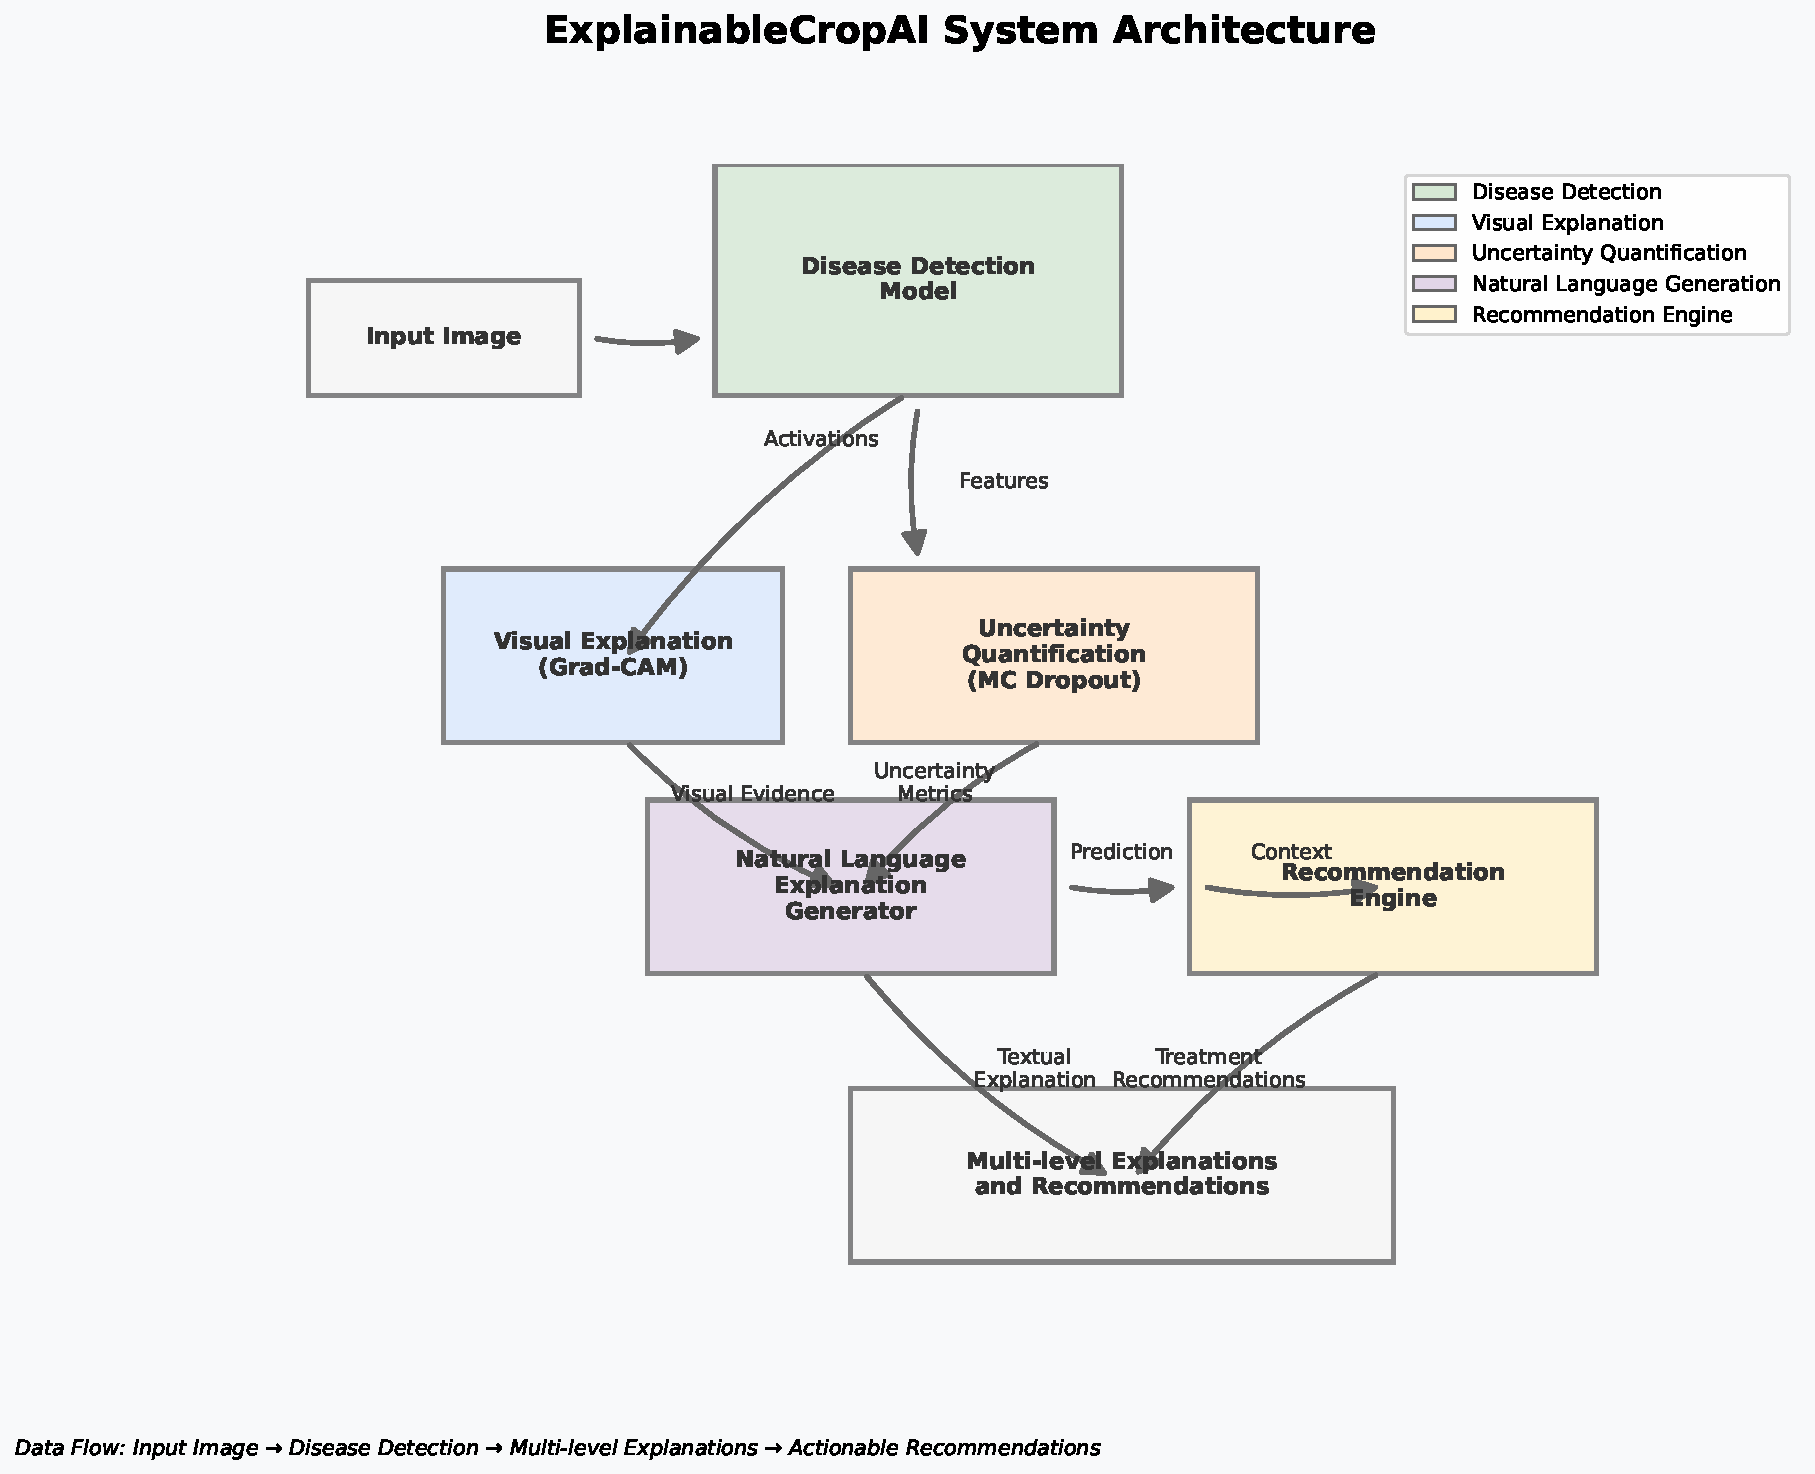
\includegraphics[width=\columnwidth]{../results/figures/system_architecture.pdf}
    \caption{ExplainableCropAI system architecture showing the interconnection between disease detection model, explanation components, uncertainty quantification, and recommendation system.}
    \label{fig:system-architecture}
\end{figure}

% Explanation Process Flowchart Figure
\begin{figure}[t]
    \centering
    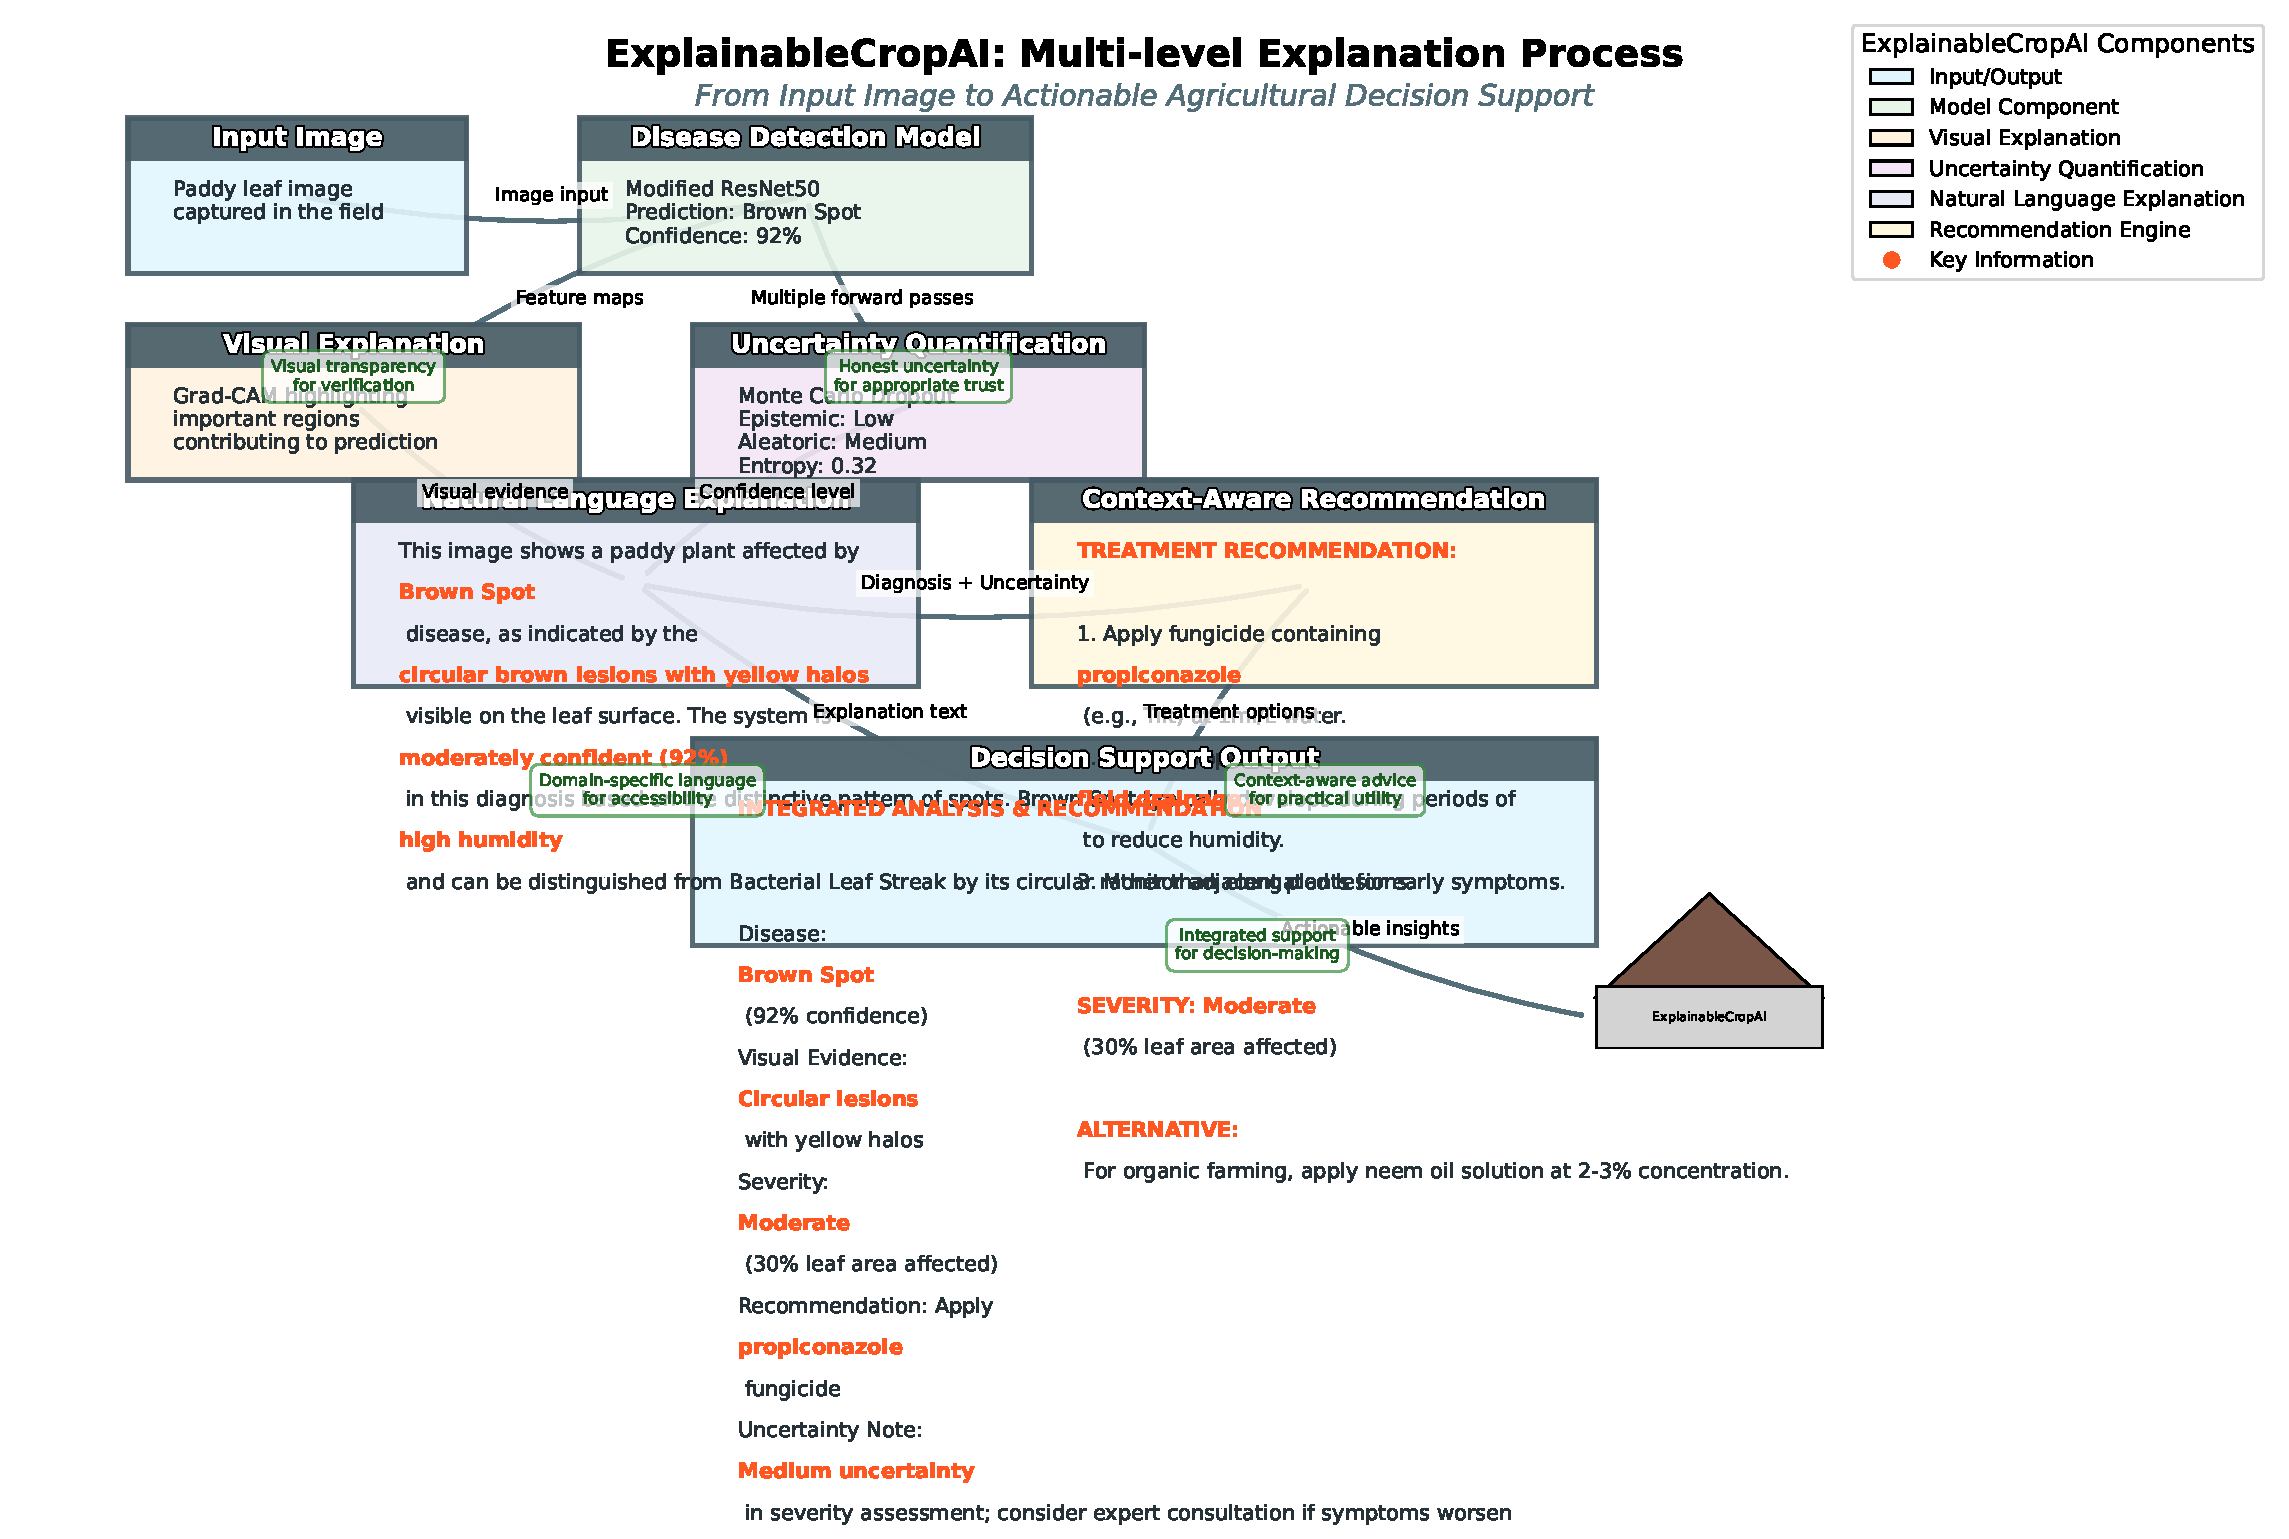
\includegraphics[width=\columnwidth]{../results/figures/explanation_flowchart.pdf}
    \caption{End-to-end explanation process in ExplainableCropAI: from input image to multi-level explanations and actionable recommendations. The flowchart illustrates how visual evidence, uncertainty information, and domain knowledge are integrated to provide comprehensive decision support.}
    \label{fig:explanation-flowchart}
\end{figure}

% Grad-CAM Examples Figure
\begin{figure}[t]
    \centering
    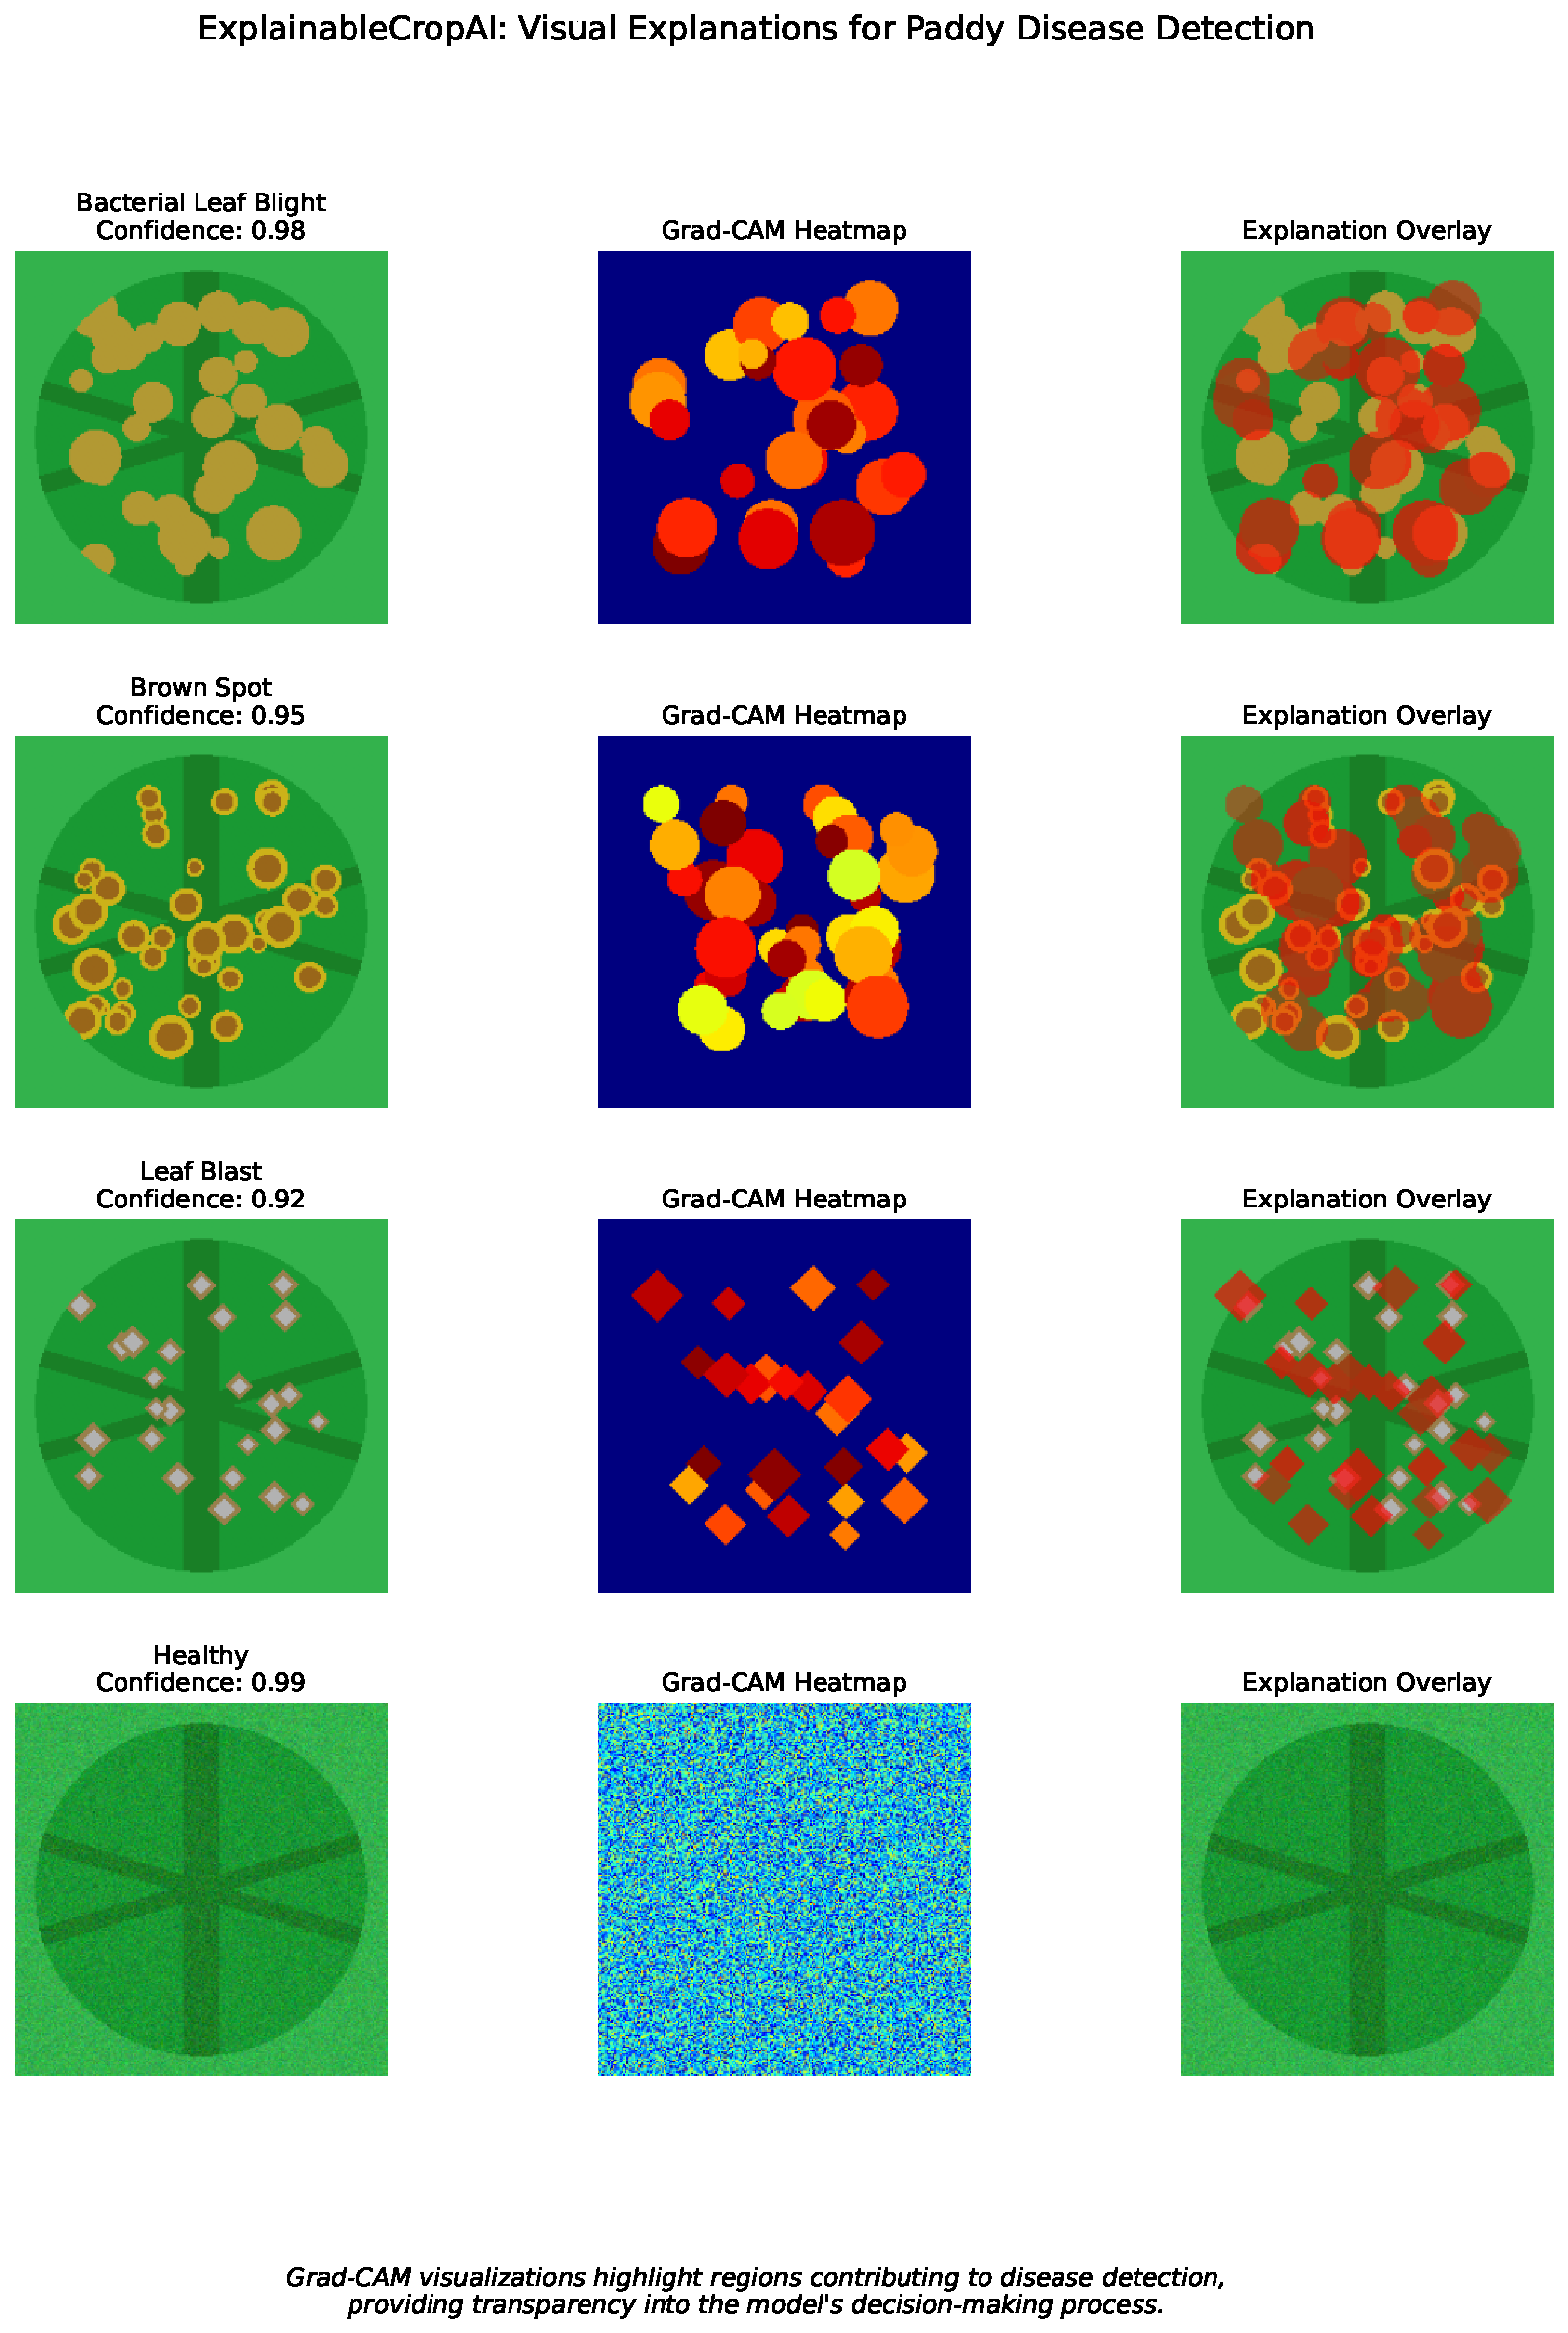
\includegraphics[width=\columnwidth]{../results/figures/gradcam_examples.pdf}
    \caption{Visual explanations generated using Grad-CAM for various paddy diseases. For each row: (left) original image, (middle) class activation heatmap, (right) heatmap overlay indicating regions contributing to the model's prediction.}
    \label{fig:gradcam-examples}
\end{figure}

% Confusion Matrix Figure
\begin{figure}[t]
    \centering
    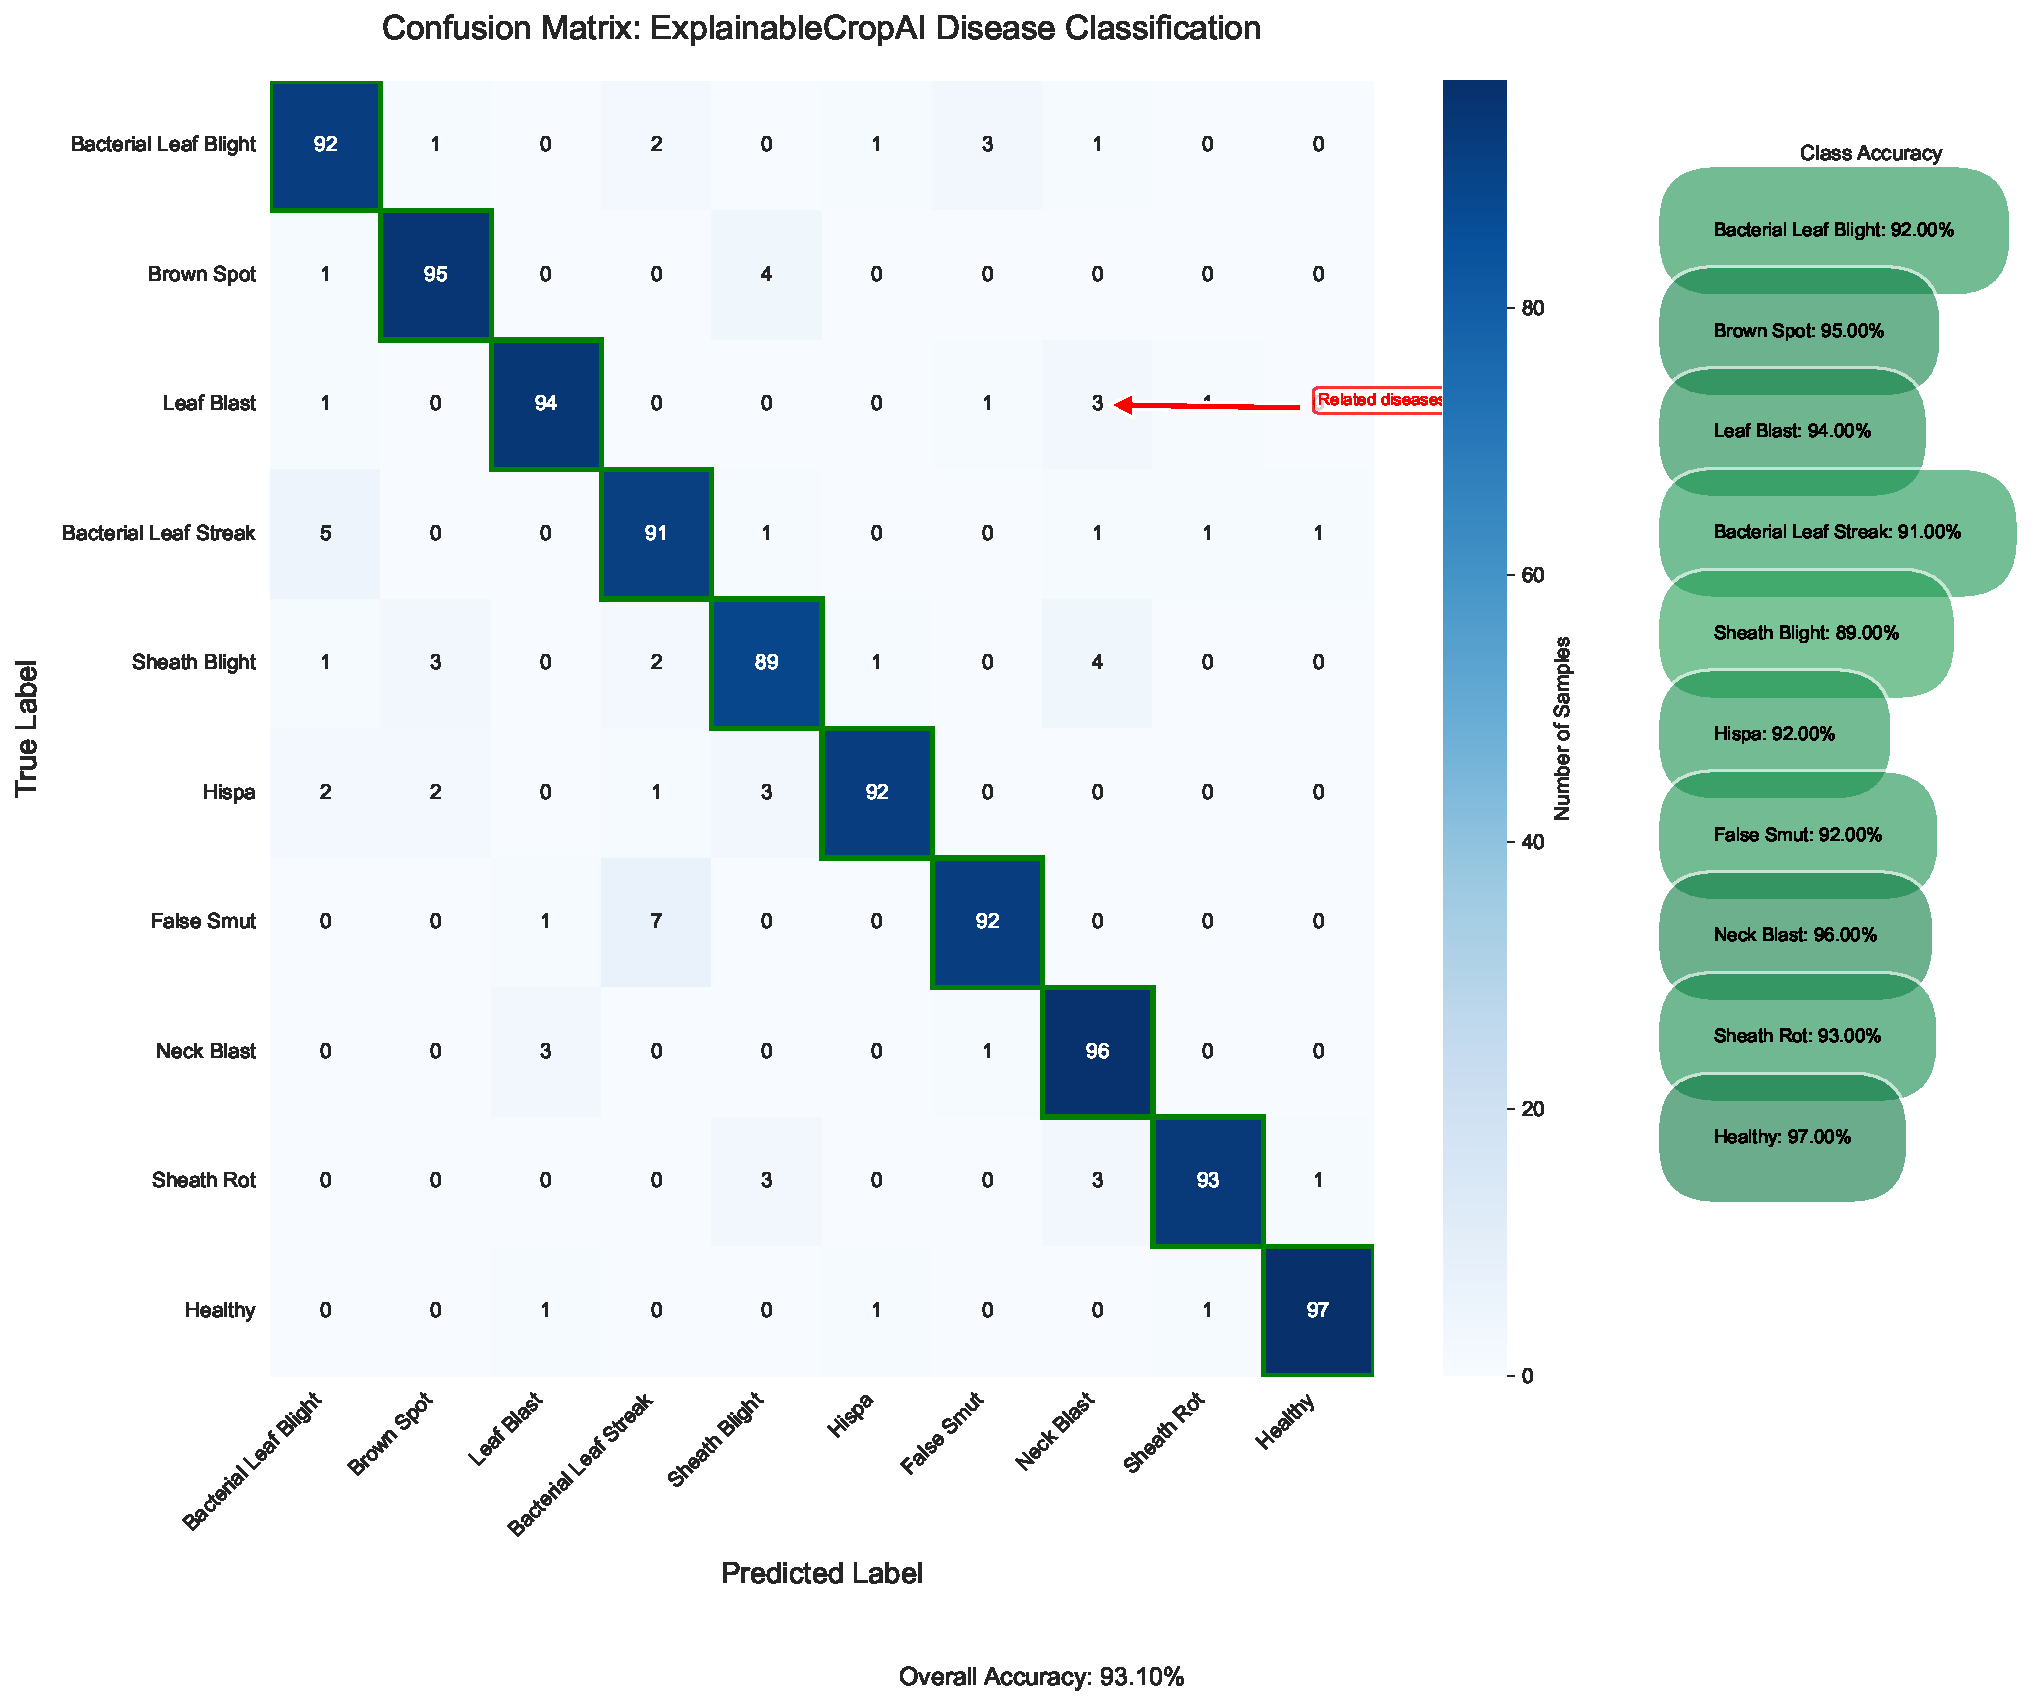
\includegraphics[width=\columnwidth]{../results/figures/confusion_matrix.pdf}
    \caption{Confusion matrix showing classification performance across ten paddy disease categories. The high values along the diagonal indicate strong classification performance, with localized confusion between visually similar diseases (e.g., Bacterial Leaf Blight and Bacterial Leaf Streak). Per-class accuracy is shown in the legend on the right.}
    \label{fig:confusion-matrix}
\end{figure}

% Uncertainty Visualization Figure
\begin{figure}[t]
    \centering
    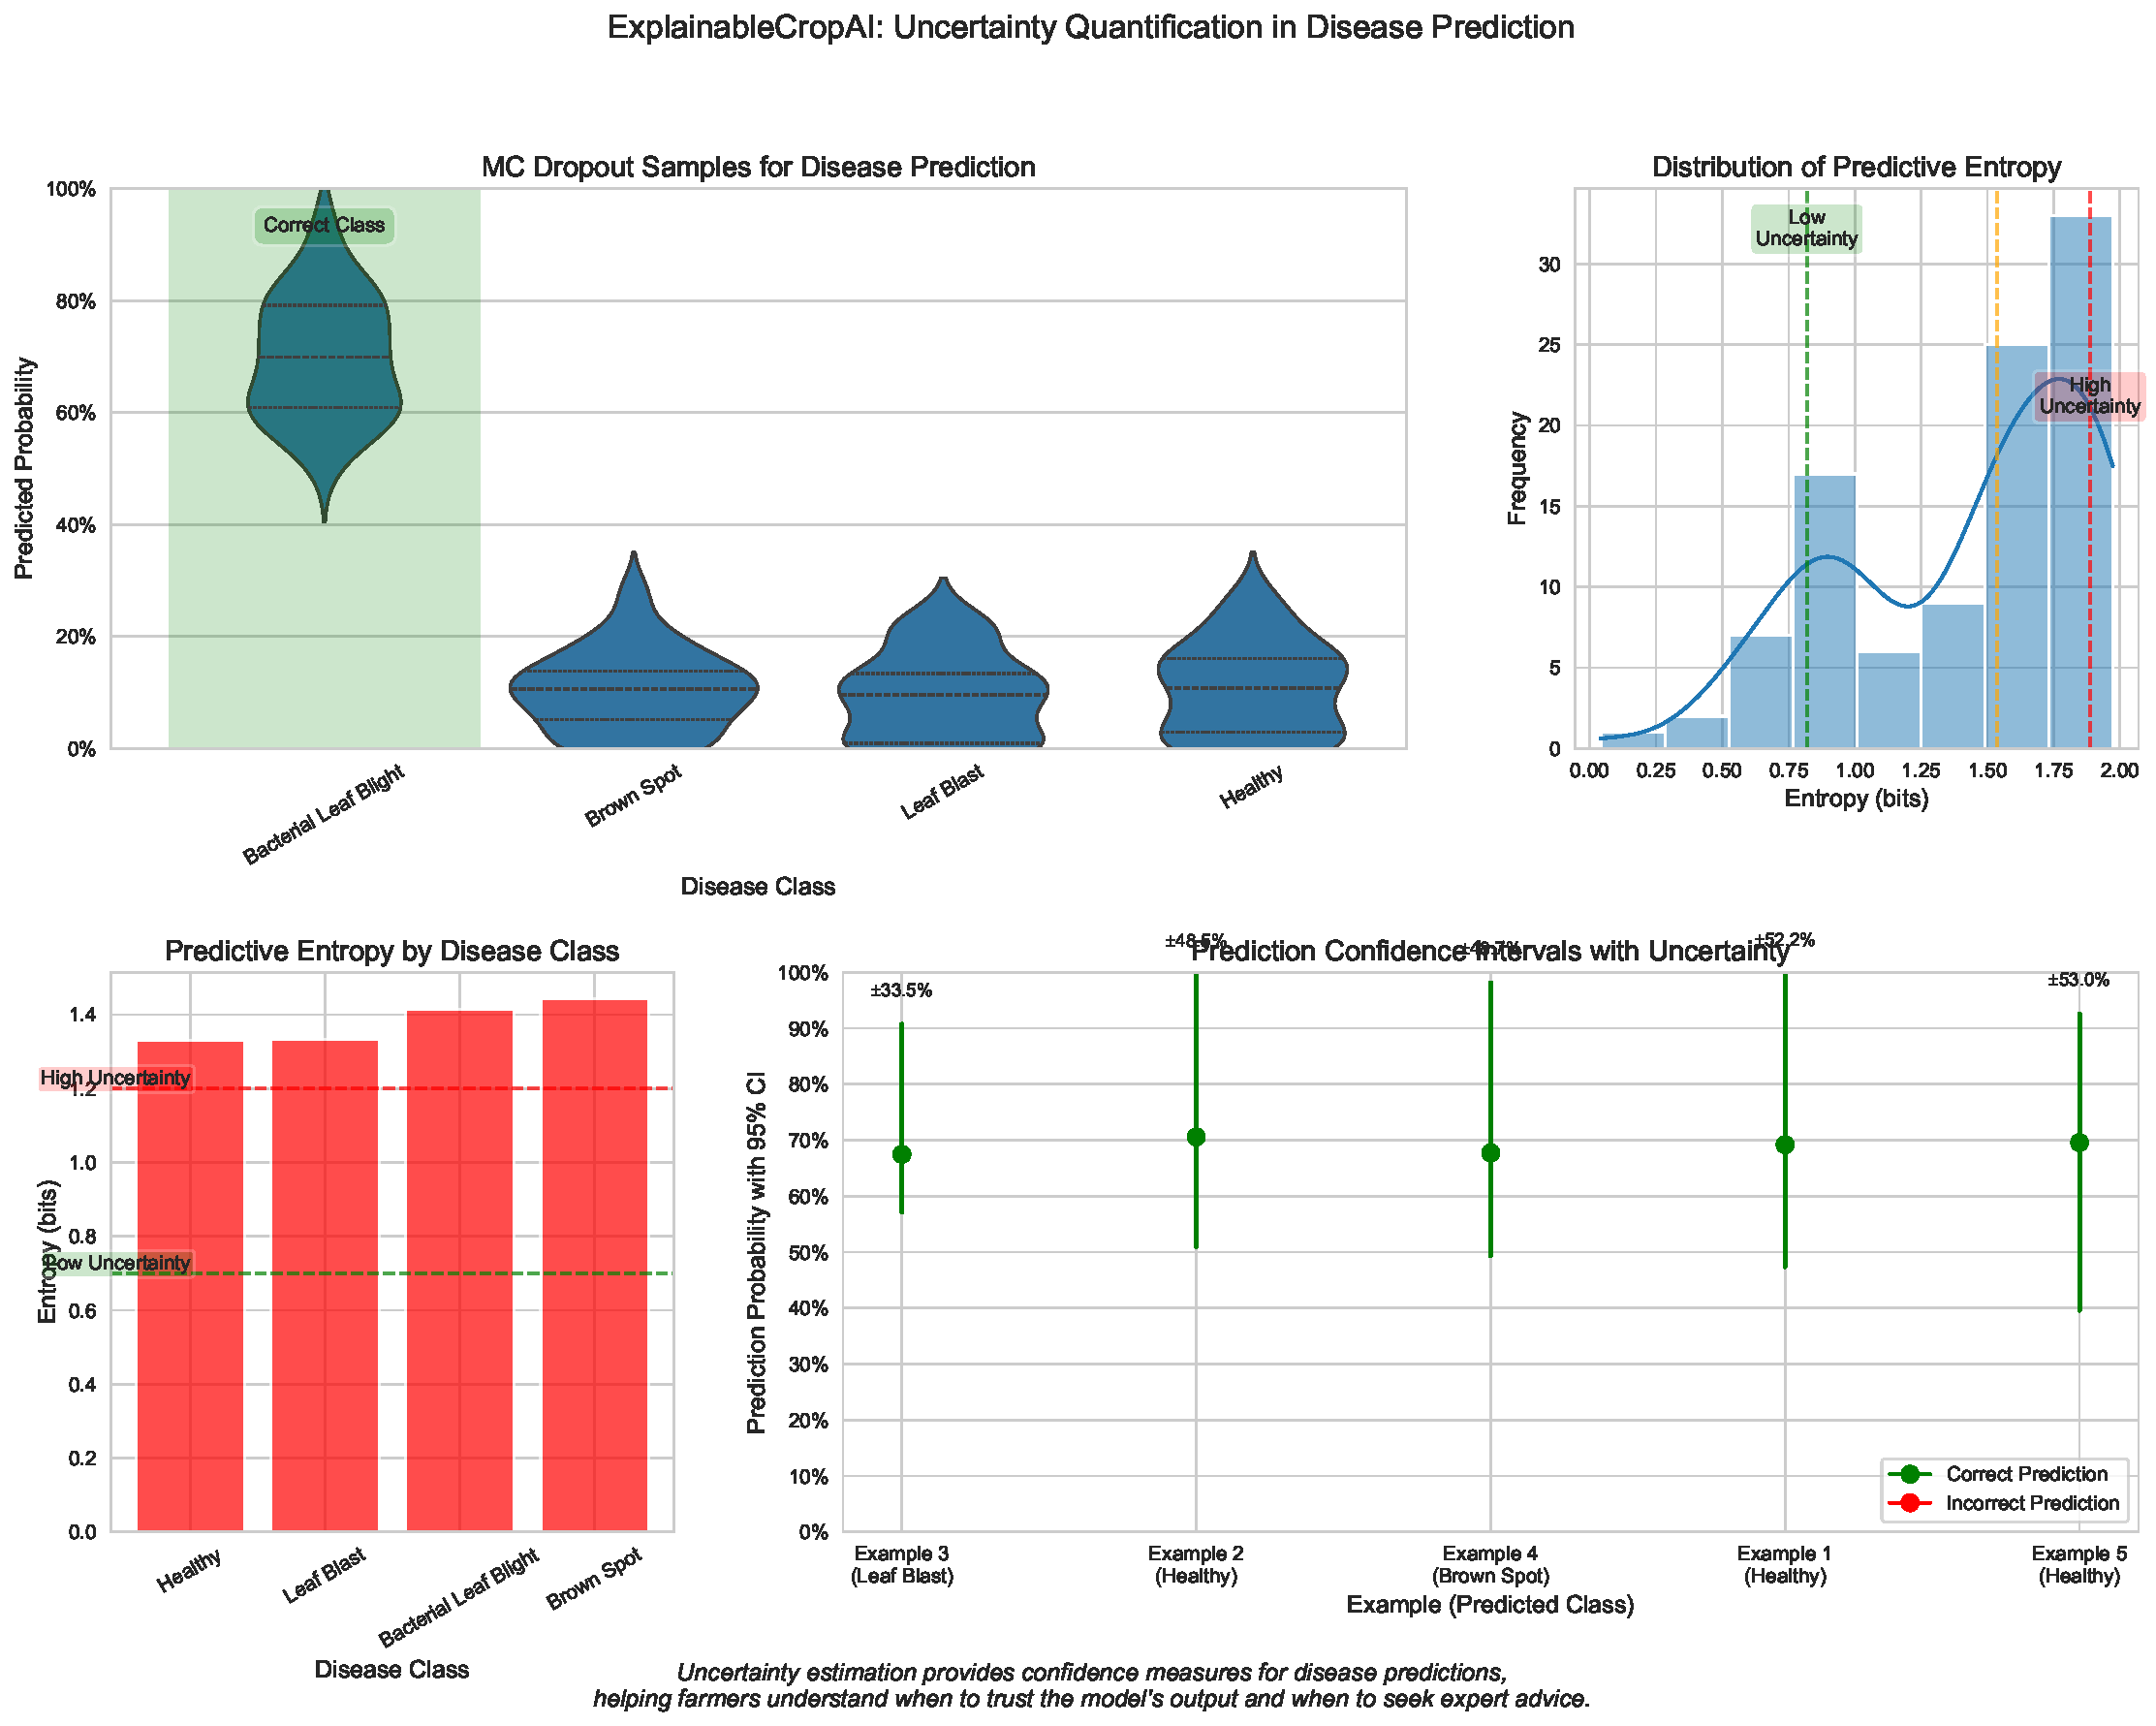
\includegraphics[width=\columnwidth]{../results/figures/uncertainty_visualization.pdf}
    \caption{Uncertainty quantification in ExplainableCropAI: (a) MC Dropout samples showing prediction distribution, (b) predictive entropy distribution indicating uncertainty levels, (c) predictive entropy by disease class, and (d) confidence intervals showing prediction uncertainty.}
    \label{fig:uncertainty-visualization}
\end{figure}

% Uncertainty-Based Recommendations Figure
\begin{figure}[t]
    \centering
    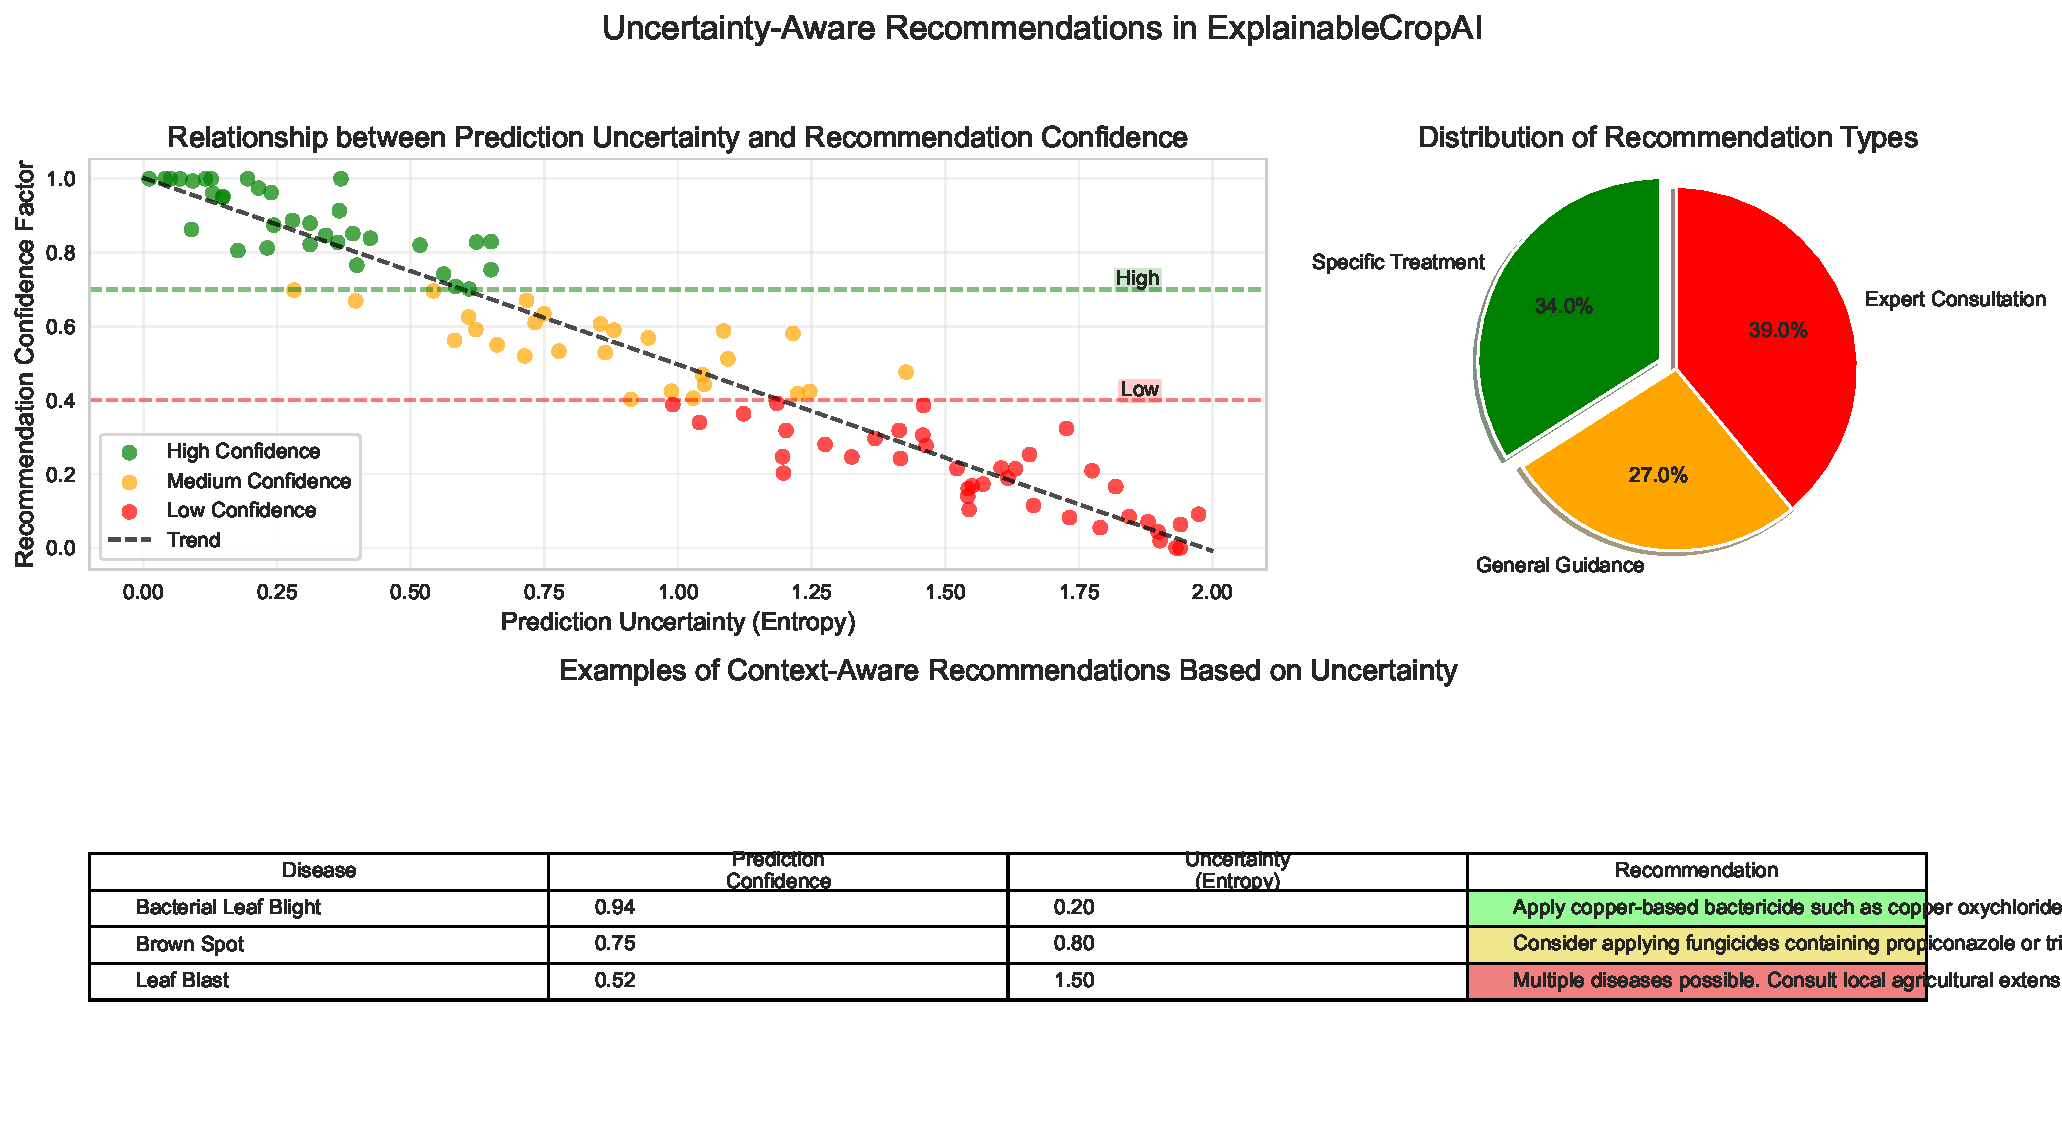
\includegraphics[width=\columnwidth]{../results/figures/uncertainty_recommendations.pdf}
    \caption{Relationship between prediction uncertainty and recommendation confidence: (a) scatter plot showing inverse correlation between uncertainty and recommendation confidence, (b) distribution of recommendation types, and (c) examples of recommendations with varying confidence levels.}
    \label{fig:uncertainty-recommendations}
\end{figure}

% User Study Results Figure
\begin{figure}[t]
    \centering
    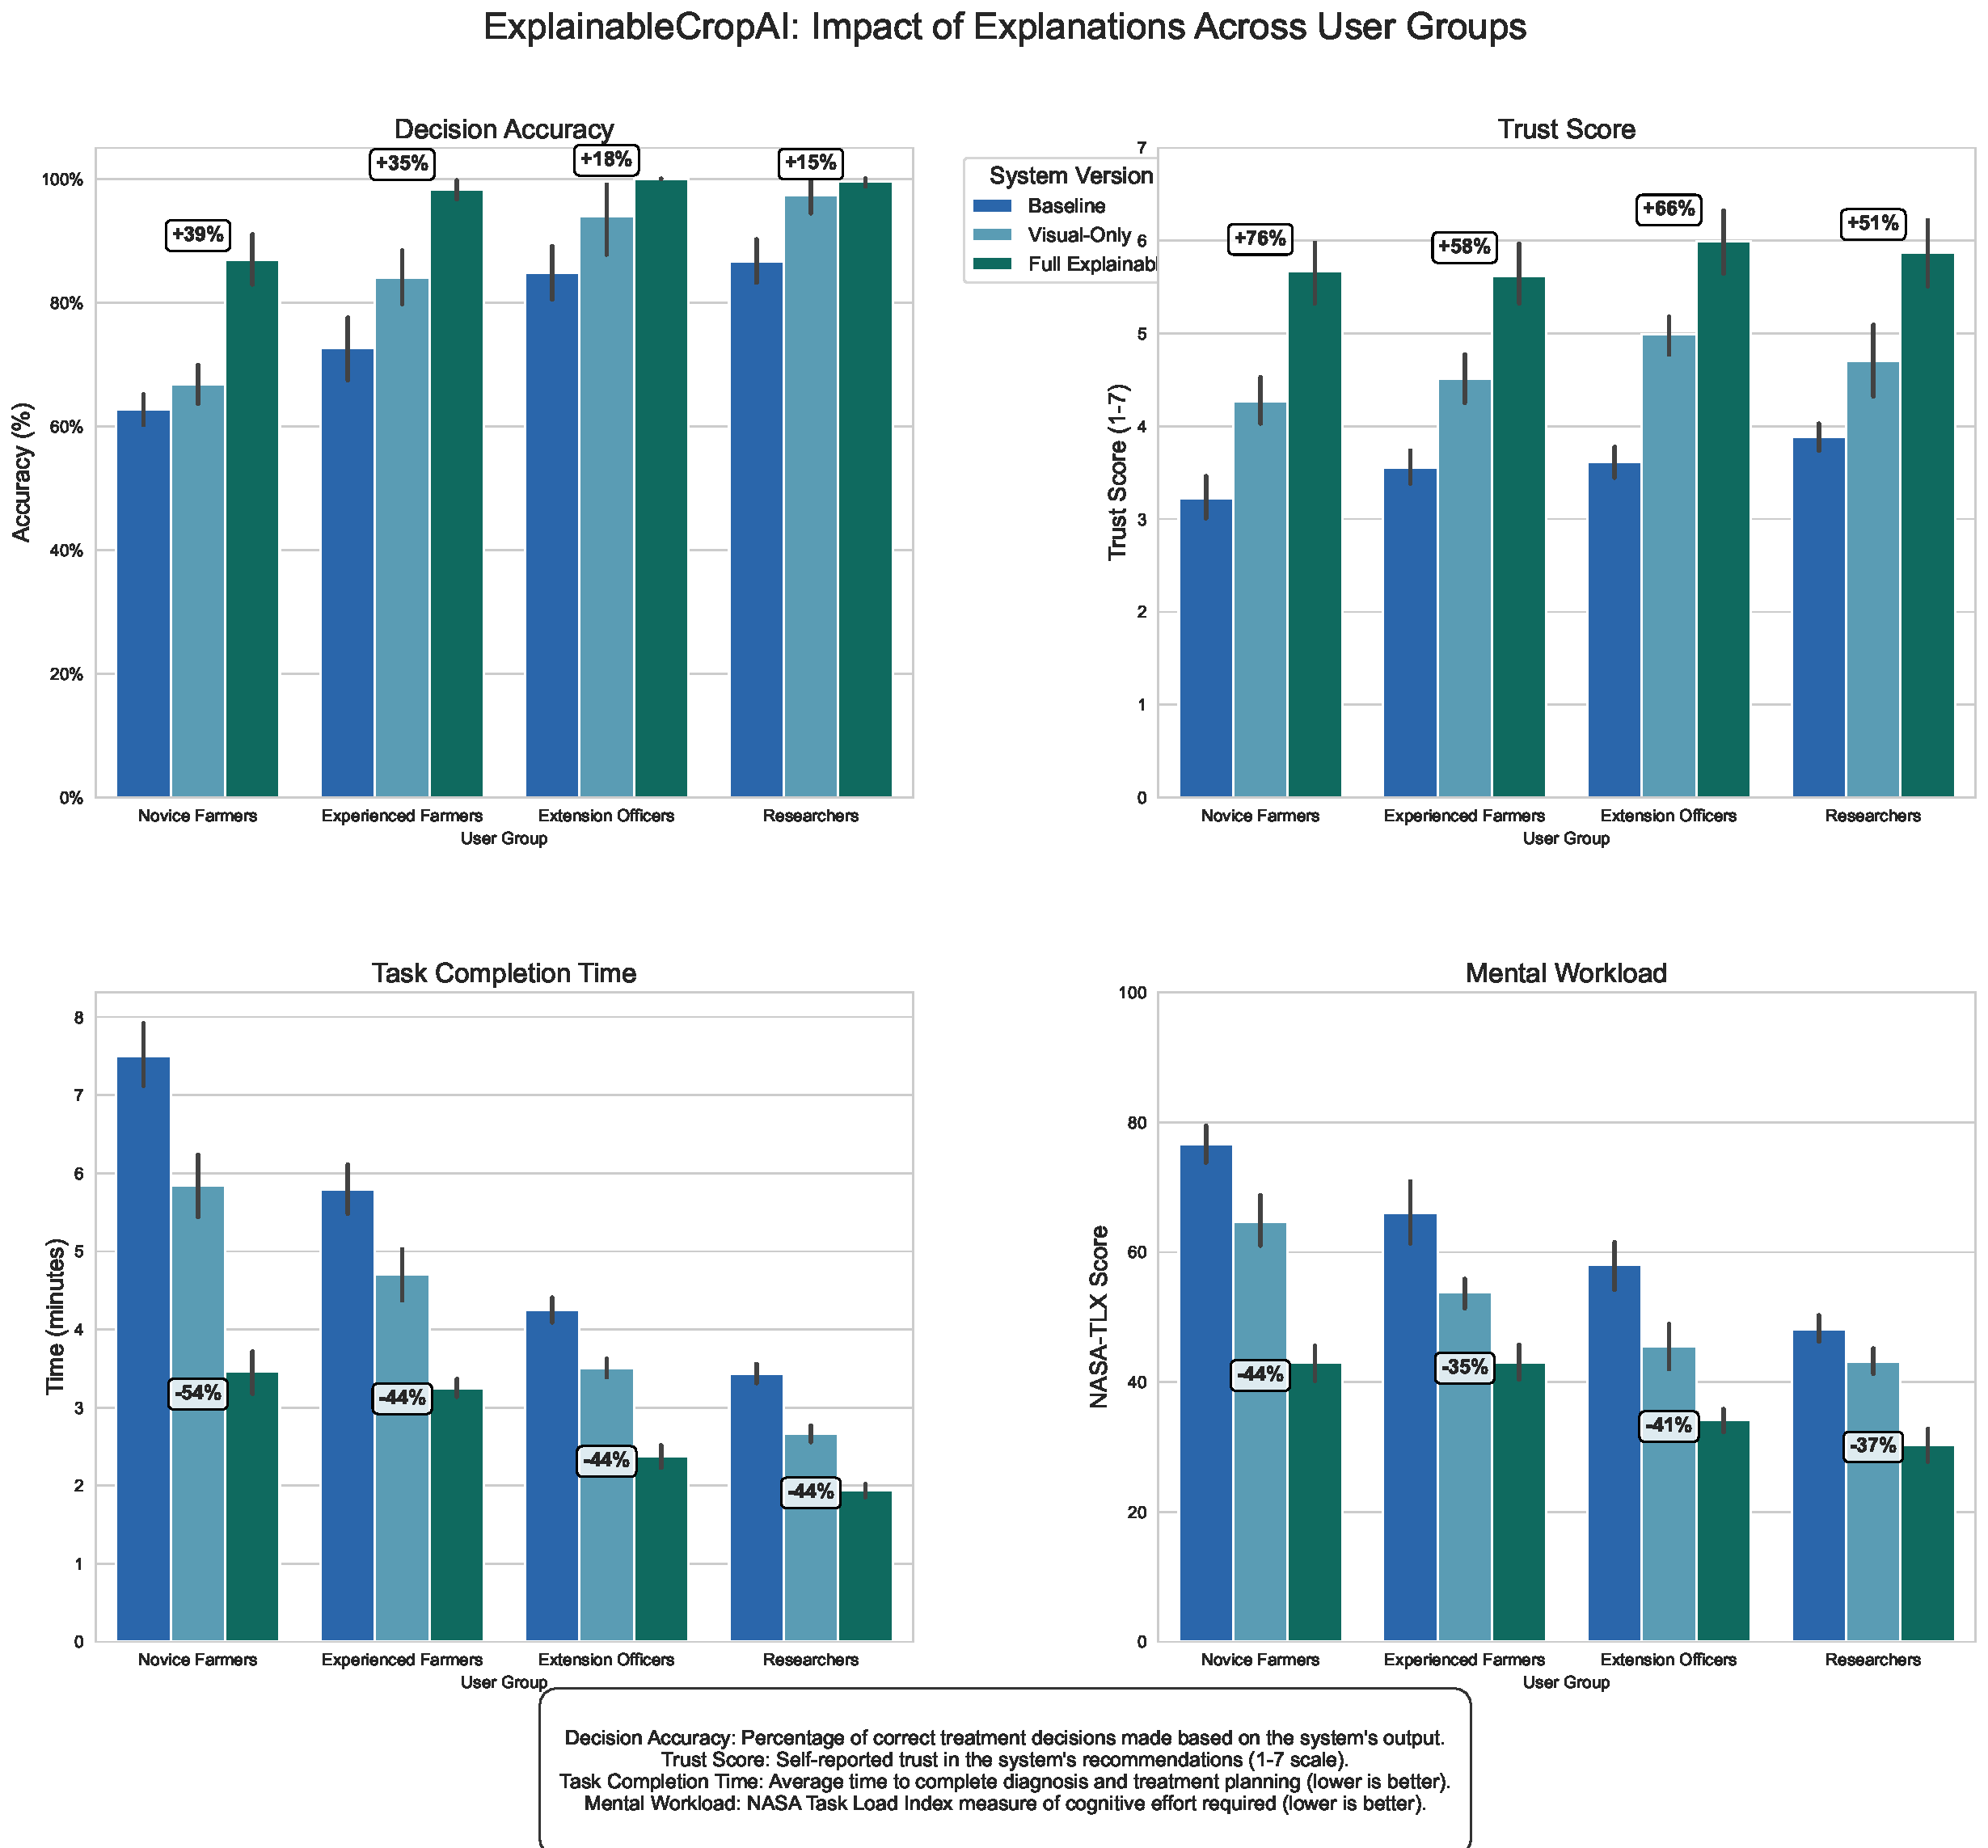
\includegraphics[width=\columnwidth]{../results/figures/user_study_results.pdf}
    \caption{Comparative analysis of ExplainableCropAI's impact across different user groups. The figure shows improvements in (a) decision accuracy, (b) trust score, (c) task completion time, and (d) mental workload when using the explanation features. Percentage improvements over the baseline are annotated for each user group, showing the differential impact of explanations based on expertise level.}
    \label{fig:user-study-results}
\end{figure}

% Explanation Effectiveness Figure
\begin{figure}[t]
    \centering
    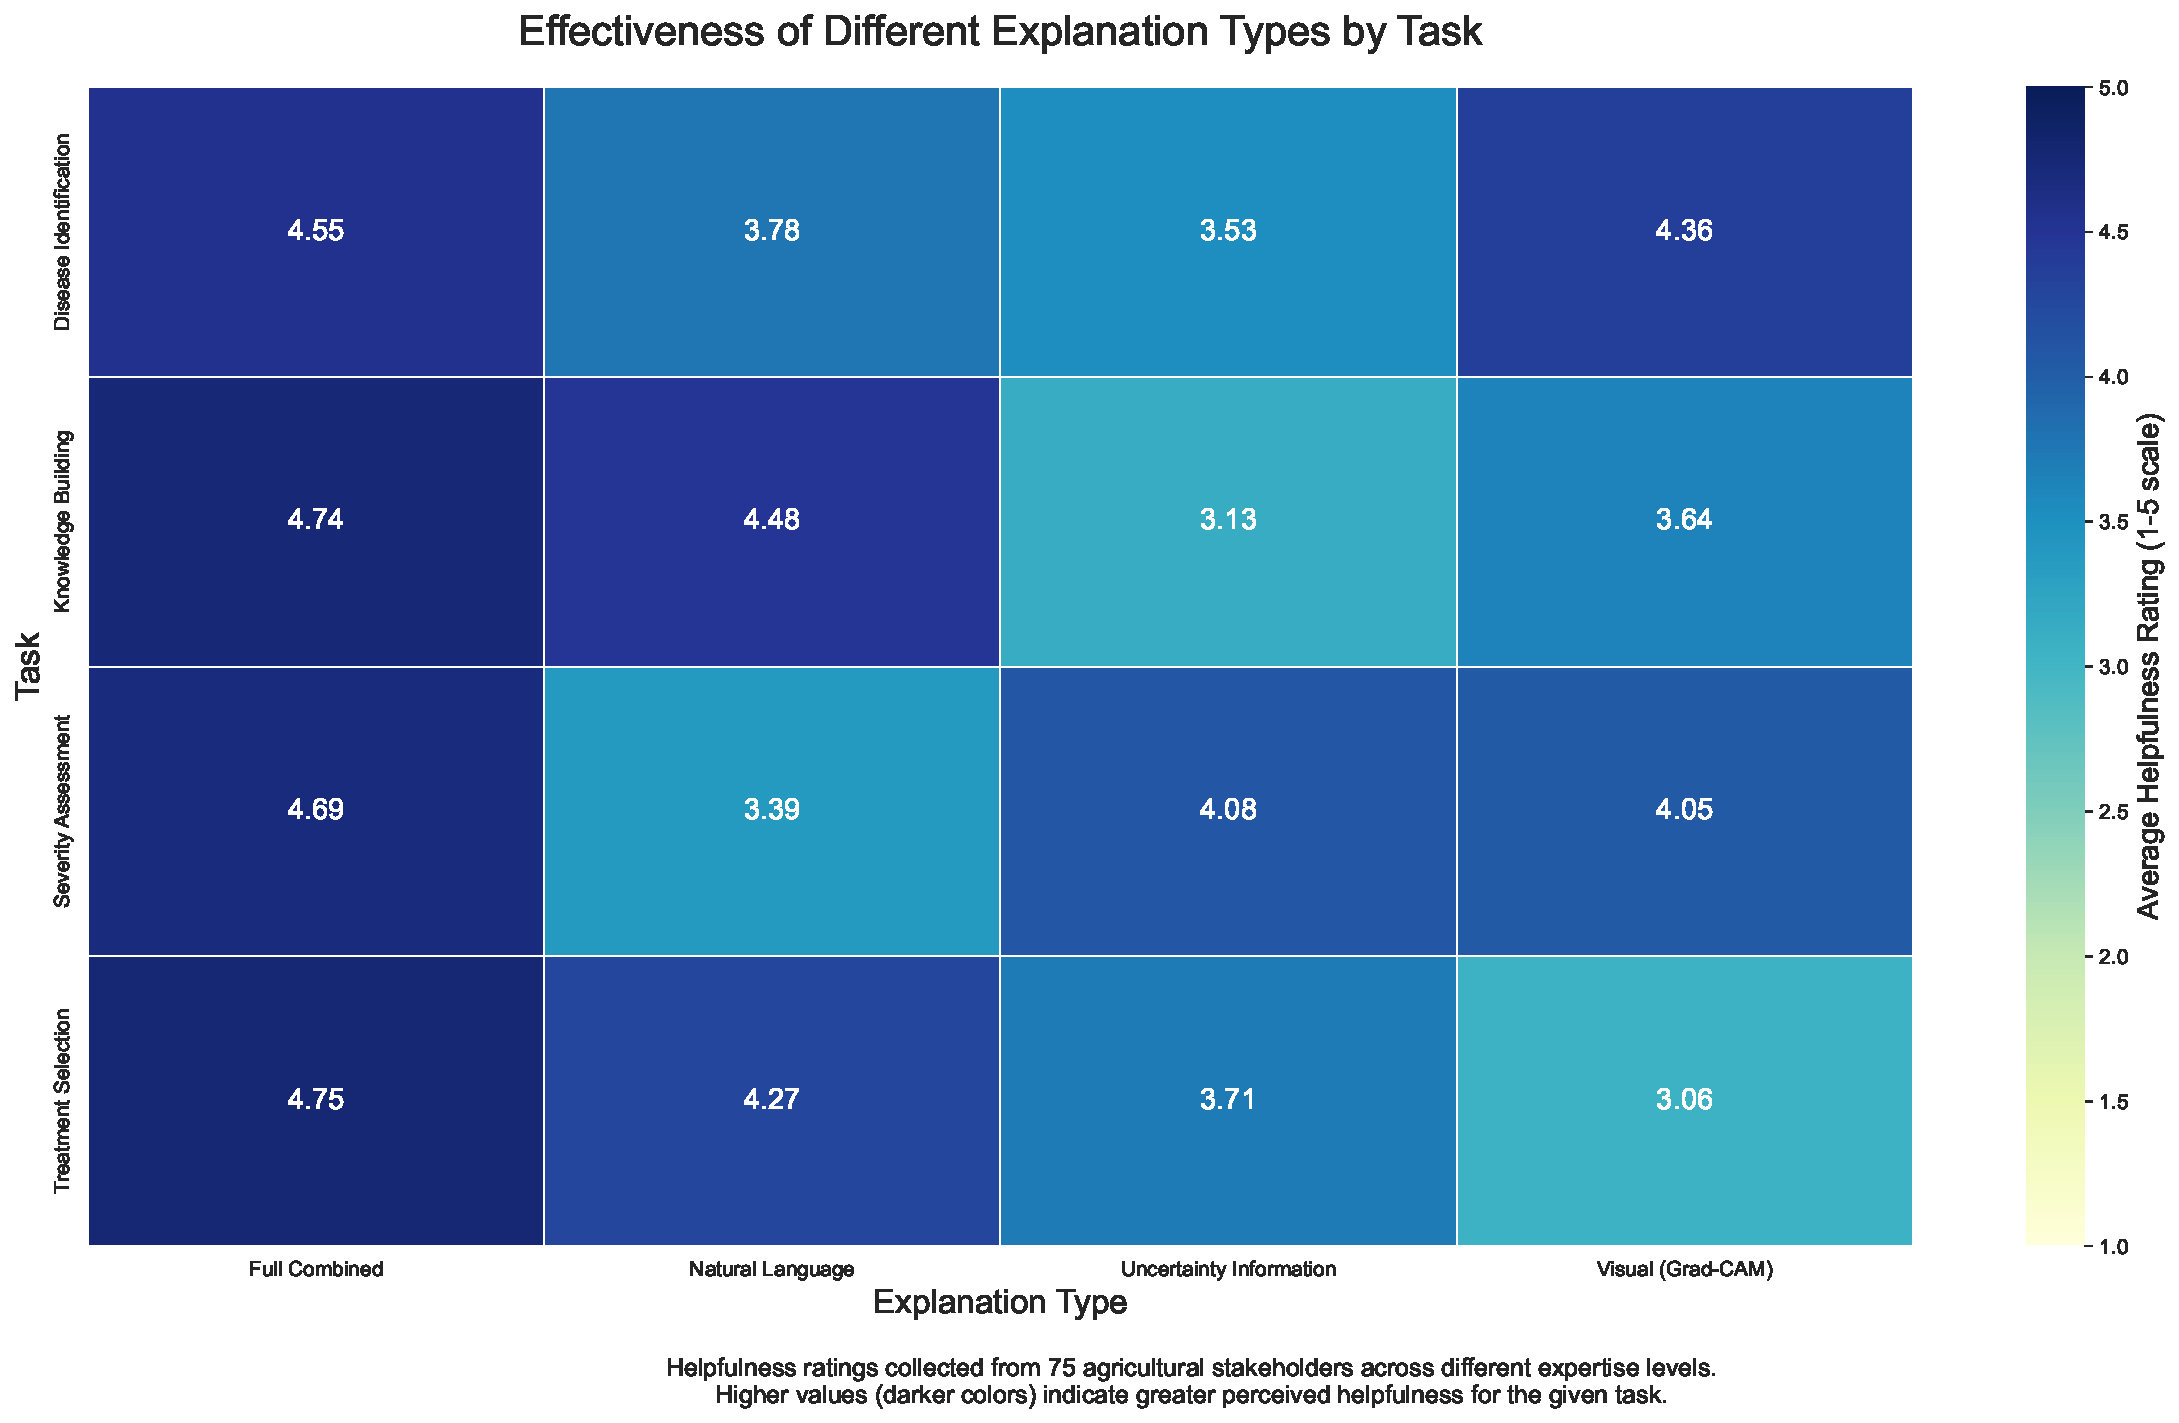
\includegraphics[width=\columnwidth]{../results/figures/explanation_effectiveness.pdf}
    \caption{Effectiveness of different explanation types across agricultural tasks. The heatmap shows average helpfulness ratings (1-5 scale) from 75 agricultural stakeholders. Natural language explanations are most effective for knowledge building and treatment selection, while visual explanations excel in disease identification, and uncertainty information is particularly valuable for severity assessment.}
    \label{fig:explanation-effectiveness}
\end{figure}

% User Interface Figure
\begin{figure}[t]
    \centering
    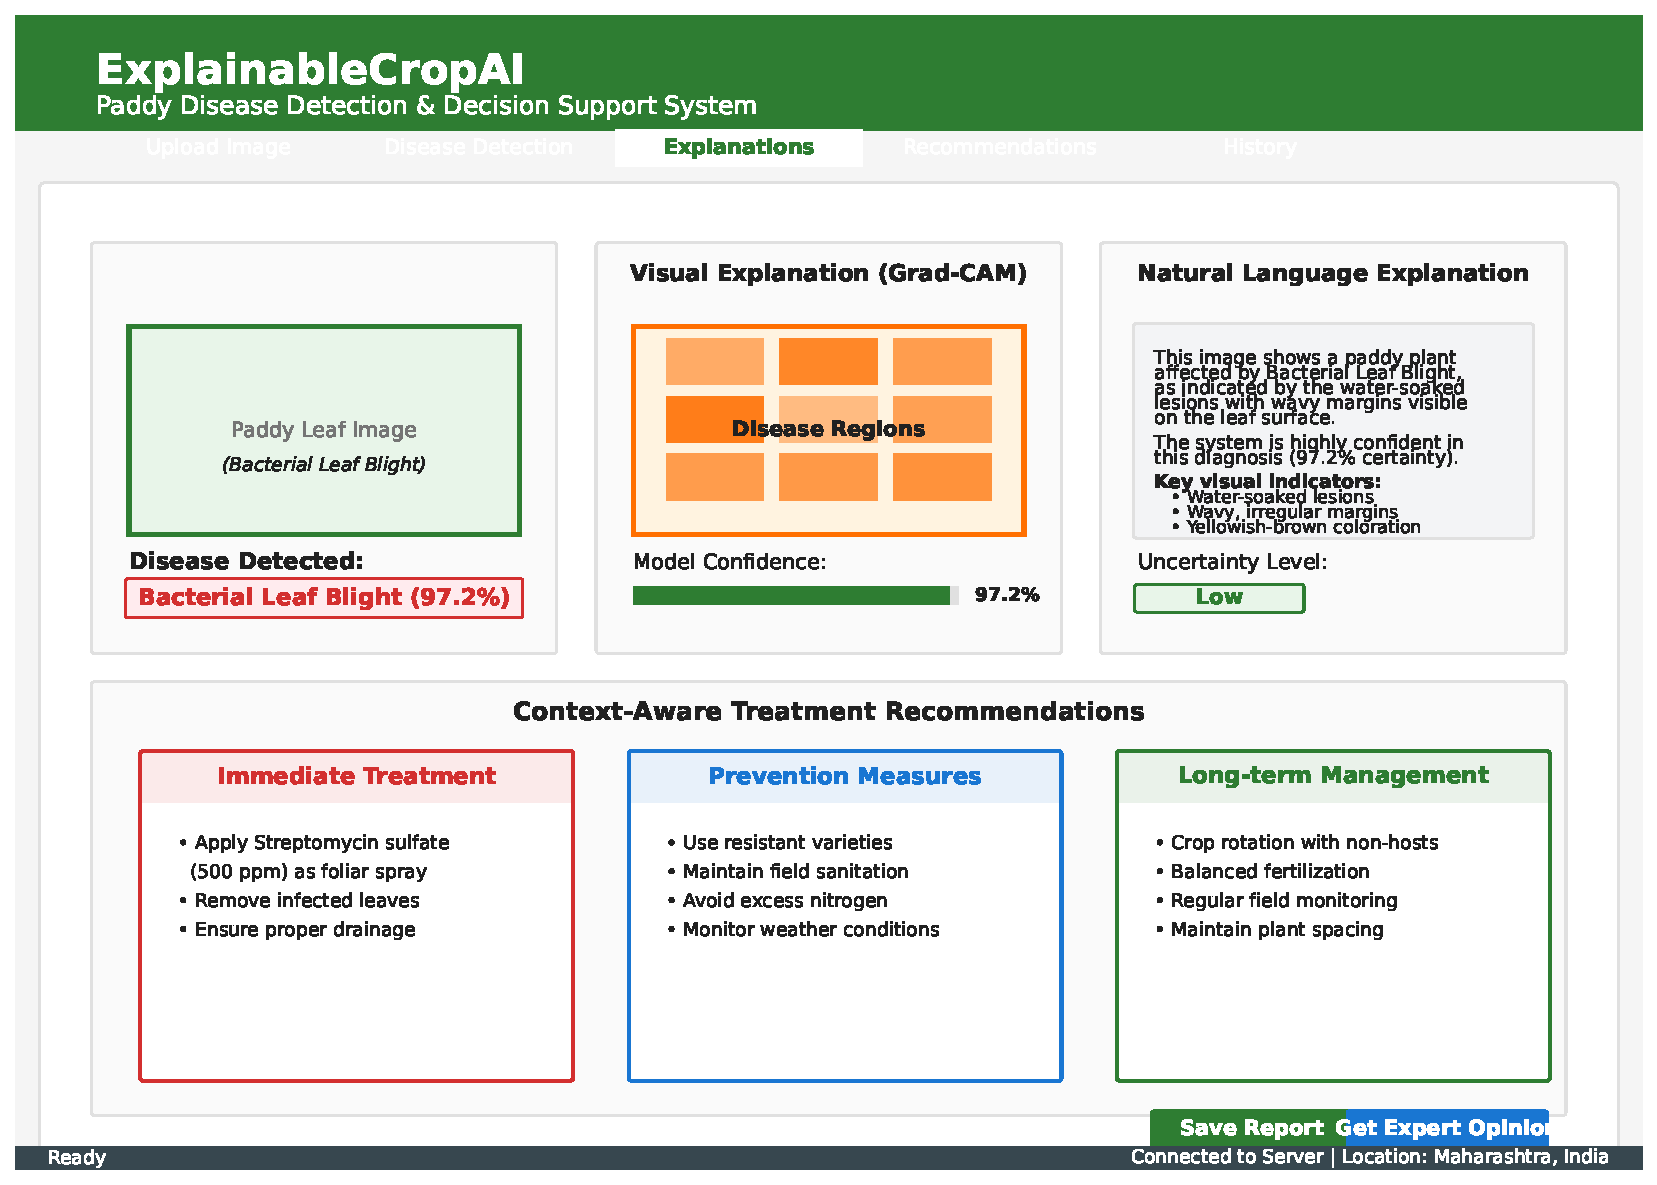
\includegraphics[width=\columnwidth]{../results/figures/user_interface.pdf}
    \caption{ExplainableCropAI user interface showing integrated prediction, explanation, and recommendation components for a detected case of Bacterial Leaf Blight. The interface provides visual explanations, natural language descriptions, uncertainty indicators, and context-aware treatment recommendations.}
    \label{fig:user-interface}
\end{figure}
